%$Header: /home/dashley/cvsrep/uculib01/uculib01/doc/manual/c_rla1/c_rla1.tex,v 1.11 2010/01/28 21:18:33 dashley Exp $

\chapter{Rational Linear Approximation}

\label{crla1}

\section{Introduction}
%Section Tag: INT
\label{crla1:sint0}

Inexpensive microcontrollers CPUs often possess integer multiplication 
and/or division machine instructions.
These instructions are always faster and more compact than corresponding
integer multiplication and division subroutines written without the
machine instructions.

In the case a processor possesses both integer multiplication and integer division 
machine instructions, it is economical to approximate an integer-valued
function $f(x)$ of a non-negative real constant $r_I$ and an 
non-negative integer $x$ defined
by

\begin{equation}
\label{eq:crla1:sint0:01}
f(x) = \lfloor r_I x \rfloor
\end{equation}

\noindent{}by choosing a non-negative integer $h$ and 
a positive integer $k$ so as to place
the rational number $r_A$ close to $r_I$\@.
(\ref{eq:crla1:sint0:01}) can then be
approximated by

\begin{equation}
\label{eq:crla1:sint0:02}
g(x) = \lfloor r_A x \rfloor 
= \left\lfloor \frac{hx}{k} \right\rfloor. 
\end{equation}

Note that (\ref{eq:crla1:sint0:02}) can be evaluated directly
by a processor with both integer multiplication and integer division
instructions, and that the 
\emph{floor($\cdot$)} function (as only non-negative $h$, $k$, $x$ are
considered) approximates the behavior of most processor integer division
instructions, which provide a remainder separately from the quotient.

In order to control (or ``place'') 
the approximation error,
it is also possible and common to add a non-negative integer $z$ to the numerator
of the approximation to yield

\begin{equation}
\label{eq:crla1:sint0:03}
g(x) = 
\left\lfloor \frac{hx + z}{k} \right\rfloor
=
\left\lfloor r_Ax + \frac{z}{k} \right\rfloor. 
\end{equation}

In the event that the processor has an integer multiplication instruction but
no integer division instruction, it is common to choose 

\begin{equation}
\label{eq:crla1:sint0:04}
r_A = \frac{h}{2^q}
\end{equation}

\noindent{}so that the division can be implemented by a bit shifting
operation.

In the event that the processor has an integer division instruction but
no integer multiplication instruction (rare), $r_A$ can be chosen as

\begin{equation}
\label{eq:crla1:sint0:05}
r_A = \frac{2^p}{k}
\end{equation}

\noindent{}so that the multiplication can be implemented by a bit-shifting
operation.

This chapter addresses the implementation of approximations of
the form of (\ref{eq:crla1:sint0:02}).  Choosing a rational number
$r_A = h/k$ as close as possible to an arbitrary $r_I$ requires 
results from number theory (a branch of mathematics); and these
results are presented here.

%%%%%%%%%%%%%%%%%%%%%%%%%%%%%%%%%%%%%%%%%%%%%%%%%%%%%%%%%%%%%%%%%%%%%%%%%%%%%%%
%%%%%%%%%%%%%%%%%%%%%%%%%%%%%%%%%%%%%%%%%%%%%%%%%%%%%%%%%%%%%%%%%%%%%%%%%%%%%%%
%%%%%%%%%%%%%%%%%%%%%%%%%%%%%%%%%%%%%%%%%%%%%%%%%%%%%%%%%%%%%%%%%%%%%%%%%%%%%%%

\section{Nomenclature}
%Section Tag: NOM
\label{crla1:snom0}

We assume that the domain of the approximation is

\begin{equation}
\label{eq:crla1:snom0:01}
x \in [0, x_{MAX}] .
\end{equation}

\noindent{}$x_{MAX}$ may in some applications be smaller than the maximum value that 
can be represented in
the data operand to the processor's integer multiplication instruction; but
the most usual case is that $x_{MAX} = 2^w-1$, where $w$ is the number of bits
in the data operand accepted by the processor's multiplication instruction.

We also assume that $h$ (of Equation \ref{eq:crla1:sint0:02} and related
equations) is constrained by

\begin{equation}
\label{eq:crla1:snom0:02}
h \in [0, h_{MAX}] .
\end{equation}

\noindent{}The most typical constraint on $h$ is due to the size of operand
that an integer multiplication instruction will accept; but there may be other reasons
for constraining $h$ (for example, to allow an arbitrary choice of $z$ 
of Equation \ref{eq:crla1:sint0:03} without
requiring test and branch logic).

Finally, we assume that $k$ is also constrained

\begin{equation}
\label{eq:crla1:snom0:03}
k \in [1, k_{MAX}] ,
\end{equation}

\noindent{}again with the most typical reason being the size of divisor that 
a machine integer division instruction will accept.

We don't constrain $z$ except to assume that $z \geq 0$
(details of possible overflow of 
$hx+z$ are left to the programmer).


%%%%%%%%%%%%%%%%%%%%%%%%%%%%%%%%%%%%%%%%%%%%%%%%%%%%%%%%%%%%%%%%%%%%%%%%%%%%%%%
%%%%%%%%%%%%%%%%%%%%%%%%%%%%%%%%%%%%%%%%%%%%%%%%%%%%%%%%%%%%%%%%%%%%%%%%%%%%%%%
%%%%%%%%%%%%%%%%%%%%%%%%%%%%%%%%%%%%%%%%%%%%%%%%%%%%%%%%%%%%%%%%%%%%%%%%%%%%%%%

\section[Choosing $r_A = h/k \approx r_I$]
        {Choosing \mbox{\boldmath $r_A = h/k \approx r_I$}}

%Section Tag: lcr0
\label{crla1:slcr0}

This section presents the details of how to choose $r_A = h/k$ so that
it is as close as possible to $r_I$.  Proofs are generally omitted, as they
would rely on material not presented for reasons of brevity.


%%%%%%%%%%%%%%%%%%%%%%%%%%%%%%%%%%%%%%%%%%%%%%%%%%%%%%%%%%%%%%%%%%%%%%%%%%%%%%%
%%%%%%%%%%%%%%%%%%%%%%%%%%%%%%%%%%%%%%%%%%%%%%%%%%%%%%%%%%%%%%%%%%%%%%%%%%%%%%%
%%%%%%%%%%%%%%%%%%%%%%%%%%%%%%%%%%%%%%%%%%%%%%%%%%%%%%%%%%%%%%%%%%%%%%%%%%%%%%%

\subsection{The Farey Series}

%Subsection Tag: fry0
\label{crla1:slcr0:sfry0}

The \emph{Farey}\footnote{Named after geologist John Farey. whose letter about 
these series was published in the \emph{Philosophical Magazine} in 1816.} \emph{series
of order $N$},\index{Farey series} denoted $F_{N}$,\index{F@$F_N$}
is the ordered set of all irreducible
rational numbers $h/k$ in the interval
[0,1]
with denominator $k\leq N$.
As examples, the Farey series of
orders 1 through 7, $F_1$ through $F_7$, are shown
in (\ref{eq:crla1:slcr0:sfry0:eq0001a}) through (\ref{eq:crla1:slcr0:sfry0:eq0001g}).

\begin{equation}
\label{eq:crla1:slcr0:sfry0:eq0001a}
F_1  = \left\{ {\frac{0}{1},\frac{1}{1}} \right\}
\end{equation}

\begin{equation}
\label{eq:crla1:slcr0:sfry0:eq0001b}
F_2  = \left\{ {\frac{0}{1},\frac{1}{2},\frac{1}{1}} \right\}
\end{equation}

\begin{equation}
\label{eq:crla1:slcr0:sfry0:eq0001c}
F_3  = \left\{ {\frac{0}{1},\frac{1}{3},\frac{1}{2},
                \frac{2}{3},\frac{1}{1}} \right\}
\end{equation}

\begin{equation}
\label{eq:crla1:slcr0:sfry0:eq0001d}
F_4  = \left\{ {\frac{0}{1},\frac{1}{4},
                \frac{1}{3},\frac{1}{2},
                \frac{2}{3},\frac{3}{4},
                \frac{1}{1}} \right\}
\end{equation}

\begin{equation}
\label{eq:crla1:slcr0:sfry0:eq0001e}
F_5  = \left\{ {\frac{0}{1},\frac{1}{5},\frac{1}{4},
                \frac{1}{3},\frac{2}{5},\frac{1}{2},
                \frac{3}{5},\frac{2}{3},\frac{3}{4},
                \frac{4}{5},\frac{1}{1}} \right\}
\end{equation}

\begin{equation}
\label{eq:crla1:slcr0:sfry0:eq0001f}
F_6  = \left\{ {\frac{0}{1},\frac{1}{6},\frac{1}{5},
                \frac{1}{4},
                \frac{1}{3},\frac{2}{5},\frac{1}{2},
                \frac{3}{5},\frac{2}{3},
                \frac{3}{4},
                \frac{4}{5},
                \frac{5}{6},\frac{1}{1}} \right\}
\end{equation}


\begin{equation}
\label{eq:crla1:slcr0:sfry0:eq0001g}
F_7  = \left\{ {\frac{0}{1},\frac{1}{7},\frac{1}{6},\frac{1}{5},
                \frac{1}{4},\frac{2}{7},
                \frac{1}{3},\frac{2}{5},\frac{3}{7},\frac{1}{2},
                \frac{4}{7},\frac{3}{5},\frac{2}{3},
                \frac{5}{7},\frac{3}{4},
                \frac{4}{5},
                \frac{5}{6},\frac{6}{7},\frac{1}{1} } \right\}
\end{equation}

The distribution of Farey rational numbers in
[0,1] is repeated
in any
$[i,i+1]$, $i\in \vworkintset$; so that the distribution of
Farey rationals in [0,1] supplies complete
information about the distribution in
all of $\vworkrealset$.  We
occasionally abuse the proper nomenclature by referring
to sequential rational numbers outside the
interval [0,1] as Farey terms or as part of
$F_N$, which, technically, they are not.
All of the results presented in
this chapter, can be shown to apply
everywhere in $\vworkrealsetnonneg$, so this abuse
is not harmful.

It can be proved that if $h/k$ is irreducible, then 
$(h+ik)/k$ is also irreducible (i.e. the analogous terms
in $[i, i+1]$ corresponding to the Farey terms in 
$[0,1]$ are also irreducible).

Recursive formulas do exist for generating 
successive terms of the Farey series.
Given two successive terms of a Farey series of
order $N$, $h_{j-2}/k_{j-2}$ and $h_{j-1}/k_{j-1}$
(\ref{eq:crla1:slcr0:sfry0:thm:01:eq01})
and
(\ref{eq:crla1:slcr0:sfry0:thm:01:eq02}) 
can be applied to generate the next term, 
$h_{j}/k_{j}$\@.  In applying
(\ref{eq:crla1:slcr0:sfry0:thm:01:eq01})
and
(\ref{eq:crla1:slcr0:sfry0:thm:01:eq02}), the
two terms used as input must be irreducible.

\begin{equation}
\label{eq:crla1:slcr0:sfry0:thm:01:eq01}
h_{j}  = \left\lfloor {\frac{{k_{j-2}
     + N}}{{k_{j - 1} }}} \right\rfloor h_{j - 1}  - h_{j-2}
\end{equation}

\begin{equation}
\label{eq:crla1:slcr0:sfry0:thm:01:eq02}
k_{j}  = \left\lfloor {\frac{{k_{j-2}  + N}}{{k_{j
     - 1} }}} \right\rfloor k_{j - 1}  - k_{j-2}
\end{equation}

Similarly, given two successive terms of a Farey series of
order $N$, $h_{j+1}/k_{j+1}$ and $h_{j+2}/k_{j+2}$
(\ref{eq:crla1:slcr0:sfry0:thm:01:eq03})
and
(\ref{eq:crla1:slcr0:sfry0:thm:01:eq04}) 
can be applied to generate the preceding term, 
$h_{j}/k_{j}$\@.  Again, in applying
(\ref{eq:crla1:slcr0:sfry0:thm:01:eq03})
and
(\ref{eq:crla1:slcr0:sfry0:thm:01:eq04}), the
two terms used as input must be irreducible.

\begin{equation}
\label{eq:crla1:slcr0:sfry0:thm:01:eq03}
h_j  = \left\lfloor {\frac{{k_{j + 2}  + N}}{{k_{j + 1} }}} 
\right\rfloor h_{j + 1}  - h_{j + 2}
\end{equation}

\begin{equation}
\label{eq:crla1:slcr0:sfry0:thm:01:eq04}
k_j  = \left\lfloor {\frac{{k_{j + 2}  + N}}{{k_{j + 1} }}} 
\right\rfloor k_{j + 1}  - k_{j + 2}
\end{equation}

It might appear on the surface that (\ref{eq:crla1:slcr0:sfry0:thm:01:eq01})
through (\ref{eq:crla1:slcr0:sfry0:thm:01:eq04}) provide a viable 
method for finding best rational approximations (i.e.
start with $0/1$ and $1/N$ and generate successive terms until
$r_I$ is bracketed), but in fact they do not.
The number of terms in the Farey series is approximately quadratic with
respect to the order of the series, and so generating terms starting at
an integer boundary is $O(N^2)$ and doesn't scale up well 
finding best rational approximations for processors that can
operate on 32- and 64-bit integers.

The Farey series has a convenient and intuitive graphical interpretation
involving the integer lattice\index{integer lattice}\index{lattice}%
\index{Farey series!integer lattice interpretation}
(see Fig. \ref{fig:crla1:slcr0:sfry0:00},
which illustrates this interpretation, but with $h$
also restricted).
[By integer lattice, we mean the $\vworkrealset{}^2$ plane
with each point $(x,y)$, $x,y \in \vworkintset$, marked.]
In such an interpretation, each rational number $h/k$ corresponds to
a point $(k,h)$ which is $h$ units above and $k$ units 
to the right of the origin.

\begin{figure}
\centering
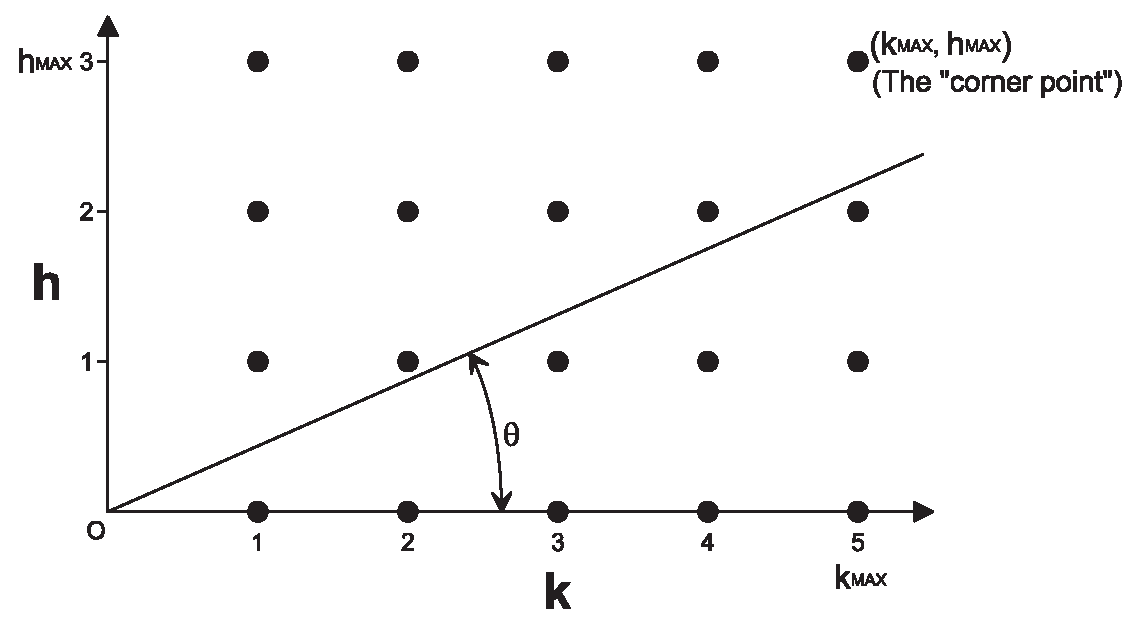
\includegraphics[width=4.6in]{c_rla1/farey01a.eps}
\caption{Graphical Interpretation Of Rational Numbers 
         $h/k$ That Can Be Formed With $h \leq h_{MAX}=3$, $k \leq k_{MAX}=5$}
\label{fig:crla1:slcr0:sfry0:00}
\end{figure}

From the graphical interpretation suggested by Fig. \ref{fig:crla1:slcr0:sfry0:00},
the following properties are intuitively clear.

\begin{itemize}
   \item The angle of a ray drawn from the origin to the point
         $(k,h)$ corresponding to the rational number $h/k$ is
         $\theta = tan^{-1} \; h/k$.

   \item Any integer lattice point on a line from 
         the origin drawn at the angle $\theta$
         has the value $h/k = tan \; \theta$.  All points corresponding
         to rational numbers with the same value will be on such a line,
         and thus form an equivalence class.

   \item A rational number $h/k$ is irreducible if and only if its corresponding
         point $(k,h)$ is ``directly'' visible from the origin with
         no intervening points.

   \item The Farey series of order $N$, $F_N$, can be 
         formed graphically by starting with the
         set of integer lattice points
         $(k,h): \; h \in \vworkintsetnonneg \wedge 1 \leq k \leq N$, 
         then sweeping
         a line extended from the origin, starting with 
         angle $\theta = 0$, through
         $0 \leq \theta < \pi{}/2$, and recording 
         in order each point directly visible from
         the origin.\footnote{Note that Fig. \ref{fig:crla1:slcr0:sfry0:00},
         because it illustrates the case when $h$ is constrained
         as well, does not show integer lattice points for
         $h > h_{MAX}$.  In principle, if the integer lattice shown
         in Fig. \ref{fig:crla1:slcr0:sfry0:00} were extended indefinitely
         ``upward'', every positive irreducible rational number with
         $k \leq k_{MAX} = 5$ could be found graphically.}
\end{itemize}

Fig. \ref{fig:crla1:slcr0:sfry0:01} illustrates the graphical construction method
of $F_5$.  Note that only integer lattice points which are directly
visible from the origin (with no intervening points) are selected.
(Fig. \ref{fig:crla1:slcr0:sfry0:01}, like Fig. \ref{fig:crla1:slcr0:sfry0:00},
shows the case of constrained $h$---the integer lattice should be
continued ``upward'' to construct the Farey series.)

\begin{figure}
\centering
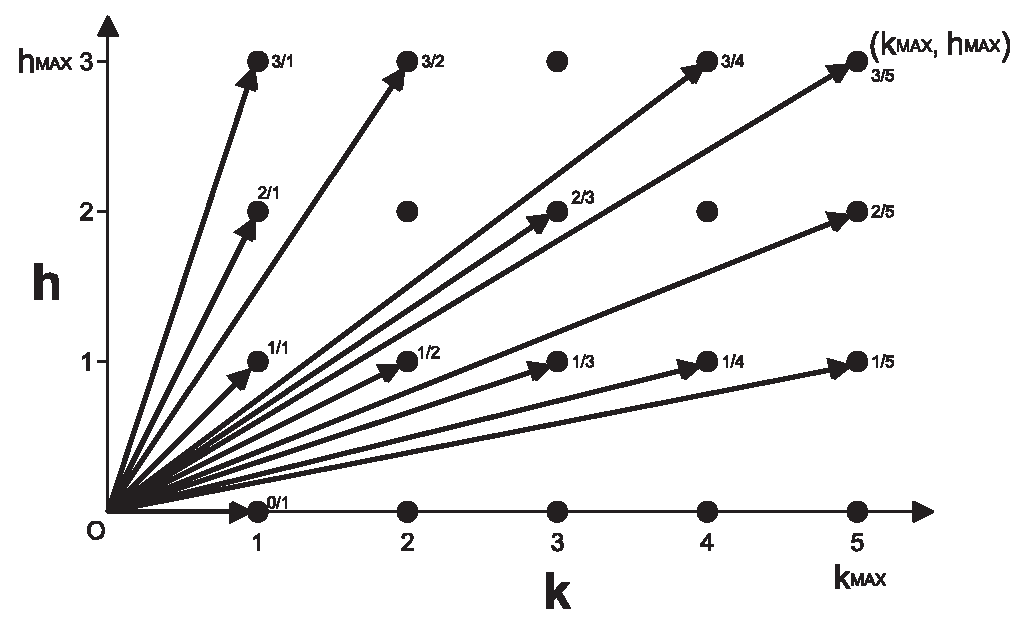
\includegraphics[width=4.6in]{c_rla1/farey01b.eps}
\caption{Graphical Interpretation Of Irreducible Rational Numbers 
         $h/k$ That Can Be Formed With $h \leq h_{MAX}=3$, $k \leq k_{MAX}=5$}
\label{fig:crla1:slcr0:sfry0:01}
\end{figure}

Note that Figures \ref{fig:crla1:slcr0:sfry0:00}
and \ref{fig:crla1:slcr0:sfry0:01} depict the case when
\emph{both} $h$ and $k$ are constrained (whereas the Farey series
constrains only $k$).

To give a compact notation, we denote the set of ascending irreducible
rational numbers that can be graphically formed
from Figures \ref{fig:crla1:slcr0:sfry0:00}
and \ref{fig:crla1:slcr0:sfry0:01} as  
$F_{k_{MAX}, h_{MAX}}$.  Using this notation, the graphical construction method
depicted in Figure \ref{fig:crla1:slcr0:sfry0:01} identifies $F_{5,3}$.

The ``corner point'' in Figures \ref{fig:crla1:slcr0:sfry0:00}
and \ref{fig:crla1:slcr0:sfry0:01} plays a special role:

\begin{itemize}
\item From 0/1 up through the corner point $h_{MAX}/k_{MAX}$,
      the terms are the terms of the Farey series of order
      $k_{MAX}$.
\item From $h_{MAX}/k_{MAX}$ up through $h_{MAX}/1$, the terms
      are the reverse-ordered reciprocals of the terms of the
      Farey series of order $h_{MAX}$.\footnote{This can be verified
      by transposing the $h$ and $k$ axes of the figures.}
\end{itemize}

As an example, $F_{5,3}$ identified graphically
is Figure \ref{fig:crla1:slcr0:sfry0:01} is

\begin{equation}
\label{eq:crla1:slcr0:sfry0:10}
F_5  = \left\{ {\frac{0}{1},\frac{1}{5},\frac{1}{4},
                \frac{1}{3},\frac{2}{5},\frac{1}{2},
                \frac{3}{5},\frac{2}{3},\frac{3}{4},
                \frac{1}{1},\frac{3}{2}, \frac{2}{1},
                \frac{3}{1} } \right\} .
\end{equation}

It can be seen by comparing (\ref{eq:crla1:slcr0:sfry0:10})
with (\ref{eq:crla1:slcr0:sfry0:eq0001c}) and 
(\ref{eq:crla1:slcr0:sfry0:eq0001e}) that the first seven terms of
(\ref{eq:crla1:slcr0:sfry0:10}) come from $F_5$ and the remaining
six terms are the reverse-ordered reciprocals of $F_3$ (although $F_3$
must be extended from Eq. \ref{eq:crla1:slcr0:sfry0:eq0001c}
into [1,2] to include 4/3 and 3/2).

The symmetry of Figures \ref{fig:crla1:slcr0:sfry0:00} and 
\ref{fig:crla1:slcr0:sfry0:01} with respect to the corner point
is important, because it means that finding best 
rational approximations for 
$r_I < h_{MAX}/k_{MAX}$ is the same problem as for 
$r_I > h_{MAX}/k_{MAX}$.  In the case of
$r_I < h_{MAX}/k_{MAX}$, the Farey series of order
$k_{MAX}$ is used, and in the case of
$r_I > h_{MAX}/k_{MAX}$ the Farey series of order
$h_{MAX}$ is used (but the reciprocals of the terms are
used, the order of the terms is reversed, and $1/r_I$ is used).  Thus, if we
know how to bracket $r_I < h_{MAX}/k_{MAX}$
in $F_{k_{MAX}}$, we can approach
the problem of $r_I > h_{MAX}/k_{MAX}$
through the inherent symmetry.


%%%%%%%%%%%%%%%%%%%%%%%%%%%%%%%%%%%%%%%%%%%%%%%%%%%%%%%%%%%%%%%%%%%%%%%%%%%%%%%
%%%%%%%%%%%%%%%%%%%%%%%%%%%%%%%%%%%%%%%%%%%%%%%%%%%%%%%%%%%%%%%%%%%%%%%%%%%%%%%
%%%%%%%%%%%%%%%%%%%%%%%%%%%%%%%%%%%%%%%%%%%%%%%%%%%%%%%%%%%%%%%%%%%%%%%%%%%%%%%

\subsection{The Continued Fraction Algorithm}

%Subsection Tag: cfr0
\label{crla1:slcr0:scfr0}

A \emph{finite simple continued fraction} is a fraction of the form

\begin{equation}
\label{eq:crla1:slcr0:scfr0:00}
a_0 + \cfrac{1}{a_1 + \cfrac{1}{a_2
    + \cfrac{1}{\;\;\;\;\;\;\;\;\;\;\;\;\;\;\ldots + \cfrac{1}{a_n}}}}
    =
    [a_0; a_1, a_2, \ldots , a_n] ,
\end{equation}

\noindent{}where $a_0 \in \vworkintsetnonneg$ and 
$a_i \in \vworkintsetpos$, $i > 0$.  Each integer
$a_i$ is called an \index{continued fraction!element}\emph{element} or
\index{continued fraction!partial quotient}\emph{partial quotient} 
of the continued fraction.
To ensure a unique representation, we require, except in the case of
the continued fraction representation of an integer,
that the final element $a_n$ not be equal
to 1.

Continued fractions are quite unwieldly to write and typeset,
and so a continued fraction in the form of (\ref{eq:crla1:slcr0:scfr0:00})
is written as $[a_0; a_1, a_2, \ldots , a_n]$.  Note that the
separator between $a_0$ and $a_1$ is a semicolon (`;'), and that all other
separators are commas (`,').  In some works, commas are used exclusively; and in
other works, the first element is $a_1$ rather than $a_0$.  Throughout this
work, the notational conventions illustrated in (\ref{eq:crla1:slcr0:scfr0:00}) are
followed.

Continued fractions can be either finite or infinite.

A finite continued fraction consists of a finite number of elements
$[a_0; a_1, a_2, \ldots , a_n]$.  It can be proved that 
every rational number corresponds to a unique
finite continued fraction\footnote{So long as the $a_n \neq 1$ convention
described earlier is followed.}, and that 
every finite continued fraction corresponds to a rational number. 

An infinite continued fraction consists of an infinite number
of elements $[a_0; a_1, a_2, \ldots]$.  Because every rational number
corresponds to a finite continued fraction, all irrational numbers have
infinite continued fraction representations.

In engineering work (and due to the general prevalence of computers
and calculators), any $r_I$ to be approximated has a known approximate
numerical value.  Even quantities that are known to be irrational (such
as $\pi$ or $\sqrt{2}$) have a numerical value known to a large number
of significant digits.  For this reason, only the numerical procedure for
obtaining the continued fraction representation of a rational number is
presented here (the symbolic procedure is not discussed).  Numerical values
are always rational (for example, 3.1415 is 31,415/10,000).

\index{continued fraction!convergent}
The \emph{kth order convergent} of a continued fraction
$[a_0; a_1, \ldots{}, a_n]$ is the irreducible rational number
corresponding to $[a_0; a_1, \ldots{}, a_k]$, $k \leq n$.
In other words, the $k$th order convergent is the irreducible rational number
corresponding to the first $k+1$ partial quotients of a 
continued fraction.\footnote{``$k+1$'' because the notational
numbering
for partial quotients starts at 0 rather than 1.} 

An $n$th order continued fraction $[a_0; a_1, \ldots{}, a_n]$
has $n+1$ convergents, $[a_0]$, 
$[a_0; a_1]$, \ldots{}, and $[a_0; a_1, \ldots{}, a_n]$.
We denote the $k$th order convergent as $s_k$, with numerator
$p_k$ and denominator $q_k$.

Without proof, we present the following algorithm, Algorithm 
\ref{alg:crla1:slcr0:scfr0:akgenalg}, for
determining the continued fraction representation (i.e. the partial
quotients) as well as the convergents of a non-negative
rational number $a/b$.

\begin{vworkalgorithmstatementpar}{Continued Fraction Representation and
                                   Convergents of 
                                   A Rational Number \mbox{\boldmath $a/b$}}
\label{alg:crla1:slcr0:scfr0:akgenalg}
\begin{alglvl0}
\item $k:=-1$.
\item $divisor_{-1} := a$.
\item $remainder_{-1} := b$.

\item Repeat

\begin{alglvl1}
\item $k := k + 1$.
\item $dividend_k := divisor_{k-1}$.
\item $divisor_k  := remainder_{k-1}$.
\item $a_k :=  dividend_k \; div \; divisor_k$.
\item $remainder_k := dividend_k \; mod \; divisor_k$.
\item If $k=0$, $p_0 = a_0$; else if $k=1$, $p_1 = a_0 a_1 + 1$; 
      else $p_i = a_i p_{i-1} + p_{i-2}$.
\item If $k=0$, $q_0 = 1$; else if $k=1$, $q_1 = a_1$; 
      else $q_i = a_i q_{i-1} + q_{i-2}$.
\end{alglvl1}

\item Until ($remainder_k = 0$).
\end{alglvl0}
\textbf{\emph{Note:}} The final $s_k = p_k / q_k$ is the irreducible
form of $a/b$.  For brevity, this is not proved here.
\end{vworkalgorithmstatementpar}
%\vworkalgorithmfooter{}
\begin{vworkexamplestatement}
\label{ex:crla1:slcr0:scfr0:01}
Find the continued fraction partial quotients and convergents of 
$67/29$.
\end{vworkexamplestatement}
\begin{vworkexampleparsection}{Solution} Table 
\ref{tbl:crla1:slcr0:scfr0:01} shows the application of 
Algorithm \ref{alg:crla1:slcr0:scfr0:akgenalg} to find the
continued fraction partial quotients and convergents of $67/29$.  From
Table \ref{tbl:crla1:slcr0:scfr0:01}, the continued fraction
representation of $67/29$ is $[2;3,4,2]$.

\begin{table}
\caption{Continued Fraction Partial Quotients and Convergents of $67/29$ (Example \ref{ex:crla1:slcr0:scfr0:01})}
\label{tbl:crla1:slcr0:scfr0:01}
\begin{center}
\begin{tabular}{|c|c|c|c|c|c|c|}
\hline
\small{Index} & \small{$dividend_k$}  & \small{$divisor_k$} & \small{$a_k$}   & \small{$remainder_k$} & \small{$p_k$} & \small{$q_k$} \\
\small{($k$)} &                       &                     &                 &                       &               &               \\
\hline
\hline
\small{-1}    & \small{N/A}           & \small{67}          & \small{N/A}     & \small{29}            & \small{N/A}   & \small{N/A}   \\
\hline
\small{0}     & \small{67}            & \small{29}          & \small{2}       & \small{9}             & \small{2}     & \small{1}     \\
\hline
\small{1}     & \small{29}            & \small{9}           & \small{3}       & \small{2}             & \small{7}     & \small{3}     \\
\hline
\small{2}     & \small{9}             & \small{2}           & \small{4}       & \small{1}             & \small{30}    & \small{13}    \\
\hline
\small{3}     & \small{2}             & \small{1}           & \small{2}       & \small{0}             & \small{67}    & \small{29}    \\
\hline
\end{tabular}
\end{center}
\end{table}
\end{vworkexampleparsection}
\vworkexamplefooter{}

Finally, we present without proof a theorem that indicates how to bracket
a rational number $a/b$ that is not in $F_{k_{MAX}}$ with its two neighbors
in $F_{k_{MAX}}$.

\begin{vworktheoremstatementpar}{Enclosing Neighbors Of \mbox{\boldmath $x \notin F_N$} 
                                 In \mbox{\boldmath $F_N$}}
\label{thm:crla1:slcr0:scfr0:cfenclosingneighbors}
For a non-negative rational
number $a/b$\footnote{It is not required that $a/b$ be irreducible in
order to apply this theorem.
For brevity, many properties of convergents were omitted; it is provable that 
the convergents formed by Algorithm \ref{alg:crla1:slcr0:scfr0:akgenalg}
will be identical for $a/b$ and $ia/ib$.} not in
$F_N$ which has a
continued fraction representation
$[a_0;a_1,a_2,\ldots{} ,a_n]$, the
highest-order convergent $s_k = p_k/q_k$ with $q_k \leq N$ is one
neighbor\footnote{By neighbors in $F_N$ we mean the rational numbers
in $F_N$ immediately to the left and immediately to the right
of $a/b$.}
to $a/b$ in $F_N$, and the other neighbor in
$F_N$ is\footnote{Theorem \ref{thm:crla1:slcr0:scfr0:cfenclosingneighbors}
is a somewhat stronger statement about best approximations
than Khinchin makes in \cite{bibref:b:KhinchinClassic}, Theorem 15.
We were not able to locate
this theorem or a proof in print,
but this theorem is understood within the number theory community.
It appears on the Web
page of David Eppstein \cite{bibref:i:davideppstein} in the form of a
`C'-language computer program,
\texttt{http://www.ics.uci.edu/\~{}{}eppstein/numth/frap.c}.
Although
Dr. Eppstein phrases the solution in terms of modifying
a partial quotient, his approach is equivalent to
(\ref{eq:crla1:slcr0:scfr0:thm:cfenclosingneighbors:01}).}

\begin{equation}
\label{eq:crla1:slcr0:scfr0:thm:cfenclosingneighbors:01}
\frac{{\displaystyle{\left\lfloor {\frac{{N - q_{k - 1} }}{{q_k }}} \right\rfloor}
 p_k  + p_{k - 1} }}{{\displaystyle{\left\lfloor {\frac{{N - q_{k - 1} }}{{q_k }}}
 \right\rfloor} q_k  + q_{k - 1} }}.
\end{equation}
\end{vworktheoremstatementpar}
\begin{vworktheoremproof}
Omitted, as it relies on material not presented for brevity.
\end{vworktheoremproof}
\vworktheoremfooter{}

Theorem \ref{thm:crla1:slcr0:scfr0:cfenclosingneighbors}
can also be applied to find the Farey neighbors of an $a/b$ already
in $F_{k_{MAX}}$.  If Algorithm \ref{alg:crla1:slcr0:scfr0:akgenalg}
is applied to $a/b$, (\ref{eq:crla1:slcr0:scfr0:thm:cfenclosingneighbors:01})
will provide one Farey neighbor, and 
(\ref{eq:crla1:slcr0:sfry0:thm:01:eq01}) through
(\ref{eq:crla1:slcr0:sfry0:thm:01:eq04}) can be used to provide the other
Farey neighbor.  (Again, for brevity, the mathematical basis for this
is not presented.)

Many constants $r_I$ to be approximated are engineering constants based
on measurements or arbitrary conventions, and so are known or accepted to
only a finite number of significant digits.  Such constants are always
rational, and 
Algorithm \ref{alg:crla1:slcr0:scfr0:akgenalg}
and
Theorem \ref{thm:crla1:slcr0:scfr0:cfenclosingneighbors}
can be applied with no special consideration.

Some constants, however, are irrational.  The question naturally arises
of how to be sure that one is using enough decimal digits
in applying 
Algorithm \ref{alg:crla1:slcr0:scfr0:akgenalg}
and
Theorem \ref{thm:crla1:slcr0:scfr0:cfenclosingneighbors}.
The easiest approach to apply in practice\footnote{\emph{In practice}
because some theoretical results may be possible as far as how
many significant digits are always adequate or as far as other
criteria, but the approach taken here is the easiest practical one.}
is to confine the quantity of interest by an inequality and to be
sure that the results are the same at both boundaries
of the inequality.

For example, $\pi$ is a transcendental constant, so has a non-terminating
decimal representation.  $\pi$ to several digits (truncated at the
end) is 3.1415926535.  It follows that

\begin{equation}
\label{eq:crla1:slcr0:scfr0:30}
3.1415926535 < \pi < 3.1415926536
\end{equation}  

For compact notation, we denote the left limit as $r_{LEFT}$ and the
right limit by $r_{RIGHT}$.  We also make the observation that in some
applications, the interval is closed rather than open.\footnote{This depends
on how much is known about $r_I$---for example, we know that $\pi$ is irrational and
can't be equal to any rational number, but we
may not know this about other $r_I$ of interest.}  In the more
general case, $r_I$ is confined by:

\begin{equation}
\label{eq:crla1:slcr0:scfr0:30b}
r_{LEFT} \leq r_I < r_{RIGHT} .
\end{equation}  

With the the $r_I$ of interest confined as suggested in 
(\ref{eq:crla1:slcr0:scfr0:30b}), there are two easy approaches
to decide if the Farey neighbors of $r_I$ can be determined with
the information available.

\begin{enumerate}
\item \emph{Easier:} Locate the Farey neighbors $h_L/k_L$ and $h_R/k_R$ of
      $r_{LEFT}$, then numerically determine whether 
      $h_L/k_L \leq r_{RIGHT} \leq h_R/k_R$.
\item \emph{Harder:} Determine whether $r_{LEFT}$ and $r_{RIGHT}$ have the
      same convergents up through $p_k/q_k$ with $q_k \leq N$.  If so,
      $r_{LEFT}$ and $r_{RIGHT}$ have the same Farey neighbors.
\end{enumerate}

\noindent{}If 
Algorithm \ref{alg:crla1:slcr0:scfr0:akgenalg}
and
Theorem \ref{thm:crla1:slcr0:scfr0:cfenclosingneighbors} are
applied with 31415926535/10000000000 and 31415926536/10000000000 
separately and yield the same rational numbers $h_L/k_L$ and $h_R/k_R$ as 
left and right neighbors, then

\begin{equation}
\label{eq:crla1:slcr0:scfr0:31}
\frac{h_L}{k_L} < 3.1415926535 < \pi < 3.1415926536 < \frac{h_R}{k_R}
\end{equation}  

\noindent{}and it is thus confirmed that $h_L/k_L$ and $h_R/k_R$ are the left
and right neighbors of $\pi$ in the Farey series of interest.

Several examples follow which illustrate the technique and various special
cases.

\begin{vworkexamplestatement}
\label{ex:crla1:slcr0:scfr0:10}
Find the best rational approximation to $1/e$ in $F_{65535}$.
\end{vworkexamplestatement}
\begin{vworkexampleparsection}{Solution} Note that $e$ is irrational, implying
that $1/e$ is also irrational, thus a bounding technique might best be used
to ensure finding the correct Farey neighbors.  Using an ordinary scientific pocket
calculator, the displayed value of $e^{-1}$ is approximately 0.367879441171.
Allowing for some possible imprecision in the last digit\footnote{The guess at 
how accurate a calculator is likely to be is subjective.}, it is fairly safe to assume that

\begin{equation}
\label{eq:ex:crla1:slcr0:scfr0:10:01}
\frac{367879441170}{1000000000000} < \frac{1}{e} < \frac{367879441172}{1000000000000} .
\end{equation}

Table \ref{tbl:crla1:slcr0:scfr0:10a} shows the application of 
Algorithm \ref{alg:crla1:slcr0:scfr0:akgenalg} to find the
continued fraction partial quotients of the left inequality
limit, and Table Table \ref{tbl:crla1:slcr0:scfr0:10b} shows the
calculation of the convergents.  (The tables are separated due to typesetting
limitations---the partial quotients and convergents would normally be tabulated
together.)

\begin{table}
\caption{Continued Fraction Partial Quotients of $367,879,441,170/1,000,000,000,000$ (Example \ref{ex:crla1:slcr0:scfr0:10})}
\label{tbl:crla1:slcr0:scfr0:10a}
\begin{center}
\begin{tabular}{|c|c|c|c|c|}
\hline
\small{Index} & \small{$dividend_k$}      & \small{$divisor_k$}       & \small{$a_k$}   & \small{$remainder_k$}     \\
\small{($k$)} &                           &                           &                 &                           \\
\hline
\hline
\small{-1}    & \small{N/A}               & \small{367,879,441,170}   & \small{N/A}     & \small{1,000,000,000,000} \\
\hline
\small{0}     & \small{367,879,441,170}   & \small{1,000,000,000,000} & \small{0}       & \small{367,879,441,170}   \\
\hline
\small{1}     & \small{1,000,000,000,000} & \small{367,879,441,170}   & \small{2}       & \small{264,241,117,660}   \\
\hline
\small{2}     & \small{367,879,441,170}   & \small{264,241,117,660}   & \small{1}       & \small{103,638,323,510}   \\
\hline
\small{3}     & \small{264,241,117,660}   & \small{103,638,323,510}   & \small{2}       & \small{56,964,470,640}    \\
\hline
\small{4}     & \small{103,638,323,510}   & \small{56,964,470,640}    & \small{1}       & \small{46,673,852,870}    \\
\hline
\small{5}     & \small{56,964,470,640}    & \small{46,673,852,870}    & \small{1}       & \small{10,290,617,770}    \\
\hline
\small{6}     & \small{46,673,852,870}    & \small{10,290,617,770}    & \small{4}       & \small{5,511,381,790}     \\
\hline
\small{7}     & \small{10,290,617,770}    & \small{5,511,381,790}     & \small{1}       & \small{4,779,235,980}     \\
\hline
\small{8}     & \small{5,511,381,790}     & \small{4,779,235,980}     & \small{1}       & \small{732,145,810}       \\
\hline
\small{9}     & \small{4,779,235,980}     & \small{732,145,810}       & \small{6}       & \small{386,361,120}       \\
\hline
\small{10}    & \small{732,145,810}       & \small{386,361,120}       & \small{1}       & \small{345,784,690}       \\
\hline
\small{11}    & \small{386,361,120}       & \small{345,784,690}       & \small{1}       & \small{40,576,430}        \\
\hline
\small{12}    & \small{345,784,690}       & \small{40,576,430}        & \small{8}       & \small{21,173,250}        \\
\hline
\small{13}    & \small{40,576,430}       & \small{21,173,250}         & \small{1}       & \small{19,403,180}        \\
\hline
\small{14}    & \small{21,173,250}       & \small{19,403,180}         & \small{1}       & \small{1,770,070}         \\
\hline
\small{15}    & \small{19,403,180}       & \small{1,770,070}          & \small{10}      & \small{1,702,480}         \\
\hline
\small{16}    & \small{1,770,070}        & \small{1,702,480}          & \small{1}       & \small{67,590}            \\
\hline
\small{17}    & \small{1,702,480}        & \small{67,590}             & \small{25}      & \small{12,730}            \\
\hline
\small{18}    & \small{67,590}           & \small{12,730}             & \small{5}       & \small{3,940}             \\
\hline
\small{19}    & \small{12,730}           & \small{3,940}              & \small{3}       & \small{910}               \\
\hline
\small{20}    & \small{3,940}            & \small{910}                & \small{4}       & \small{300}               \\
\hline
\small{21}    & \small{910}              & \small{300}                & \small{3}       & \small{10}                \\
\hline
\small{22}    & \small{300}              & \small{10}                 & \small{30}      & \small{0}                 \\
\hline
\end{tabular}
\end{center}
\end{table}

\begin{table}
\caption{Continued Fraction Convergents of $367,879,441,170/1,000,000,000,000$ (Example \ref{ex:crla1:slcr0:scfr0:10})}
\label{tbl:crla1:slcr0:scfr0:10b}
\begin{center}
\begin{tabular}{|c|c|c|c|}
\hline
\small{Index} & \small{$a_k$} & \small{$p_k$}           & \small{$q_k$}            \\
\small{($k$)} &               &                         &                          \\
\hline
\hline
\small{-1}    & \small{N/A}   & \small{N/A}             & \small{N/A}              \\
\hline
\small{0}     & \small{0}     & \small{0}               & \small{1}                \\
\hline
\small{1}     & \small{2}     & \small{1}               & \small{2}                \\
\hline
\small{2}     & \small{1}     & \small{1}               & \small{3}                \\
\hline
\small{3}     & \small{2}     & \small{3}               & \small{8}                \\
\hline
\small{4}     & \small{1}     & \small{4}               & \small{11}               \\
\hline
\small{5}     & \small{1}     & \small{7}               & \small{19}               \\
\hline
\small{6}     & \small{4}     & \small{32}              & \small{87}               \\
\hline
\small{7}     & \small{1}     & \small{39}              & \small{106}              \\
\hline
\small{8}     & \small{1}     & \small{71}              & \small{193}              \\
\hline
\small{9}     & \small{6}     & \small{465}             & \small{1,264}            \\
\hline
\small{10}    & \small{1}     & \small{536}             & \small{1,457}            \\
\hline
\small{11}    & \small{1}     & \small{1,001}           & \small{2,721}            \\
\hline
\small{12}    & \small{8}     & \small{8,544}           & \small{23,225}           \\
\hline
\small{13}    & \small{1}     & \small{9,545}           & \small{25,946}           \\
\hline
\small{14}    & \small{1}     & \small{18,089}          & \small{49,171}          \\
\hline
\small{15}    & \small{10}    & \small{190,435}         & \small{517,656}         \\
\hline
\small{16}    & \small{1}     & \small{208,524}         & \small{566,827}          \\
\hline
\small{17}    & \small{25}    & \small{5,403,535}       & \small{14,688,331}       \\
\hline
\small{18}    & \small{5}     & \small{27,226,199}      & \small{74,008,482}       \\
\hline
\small{19}    & \small{3}     & \small{87,082,132}      & \small{236,713,777}      \\
\hline
\small{20}    & \small{4}     & \small{375,554,727}     & \small{1,020,863,590}    \\
\hline
\small{21}    & \small{3}     & \small{1,213,746,313}   & \small{3,299,304,547}    \\
\hline
\small{22}    & \small{30}    & \small{36,787,944,117}  & \small{100,000,000,000}  \\
\hline
\end{tabular}
\end{center}
\end{table}

Note that since we are finding best rational approximations
in $F_{65535}$, Theorem \ref{thm:crla1:slcr0:scfr0:cfenclosingneighbors}
requires only that we carry the tabular procedure of 
Algorithm \ref{alg:crla1:slcr0:scfr0:akgenalg} out until
$q_k \geq 65535$ ($k=15$ in this example).

By
Theorem \ref{thm:crla1:slcr0:scfr0:cfenclosingneighbors}
and
Table \ref{tbl:crla1:slcr0:scfr0:10b}, one Farey neighbor
to the left inequality limit is $p_{14}/q_{14} = 18,089/49,171$.
The other Farey neighbor is given by 
(\ref{eq:crla1:slcr0:scfr0:thm:cfenclosingneighbors:01}), with the calculation
detailed below.

\begin{equation}
\label{eq:ex:crla1:slcr0:scfr0:10:50a}
\frac{{\displaystyle{\left\lfloor {\frac{{N - q_{k - 1} }}{{q_k }}} \right\rfloor}
 p_k  + p_{k - 1} }}{{\displaystyle{\left\lfloor {\frac{{N - q_{k - 1} }}{{q_k }}}
 \right\rfloor} q_k  + q_{k - 1} }}.
\end{equation}

\begin{equation}
\label{eq:ex:crla1:slcr0:scfr0:10:50b}
= \frac{{\displaystyle{\left\lfloor {\frac{{65535 - q_{13} }}{{q_{14} }}} \right\rfloor}
 p_{14}  + p_{13} }}{{\displaystyle{\left\lfloor {\frac{{65535 - q_{13} }}{{q_{14} }}}
 \right\rfloor} q_{14}  + q_{13} }}.
\end{equation}

\begin{equation}
\label{eq:ex:crla1:slcr0:scfr0:10:50c}
= \frac{{\displaystyle{\left\lfloor {\frac{{65535 - 25946 }}{{49171 }}} \right\rfloor}
 18089  + 9545 }}{{\displaystyle{\left\lfloor {\frac{{65535 - 25946 }}{{49171 }}}
 \right\rfloor} 49171  + 25946 }}.
\end{equation}

\begin{equation}
\label{eq:ex:crla1:slcr0:scfr0:10:50d}
= \frac{9545}{25946}
\end{equation}

It can be verified by cross-multiplication that $9545/25946 > 18089/49171$, therefore

\begin{equation}
\label{eq:ex:crla1:slcr0:scfr0:10:50e}
\frac{18089}{49171} < 0.367879441170 < \frac{9545}{25946} .
\end{equation}

A similar tabulation procedure carried out with 
the right inequality limit (0.367879441172), not reproduced here for brevity,
verifies that it has the same convergents up through $s_{15}$ as the left
inequality limit.  Therefore it has the same Farey neighbors in $F_{65535}$
as the left limit, and it is established that

\begin{equation}
\label{eq:ex:crla1:slcr0:scfr0:10:50f}
\frac{18089}{49171} < 0.367879441170 < \frac{1}{e} < 0.367879441172 < \frac{9545}{25946} .
\end{equation}

It can be verified numerically that 18089/49171 and 9545/25946 are both \emph{very}
close approximations to $1/e$ (with differences on the order of a couple parts per
\emph{billion}).
\end{vworkexampleparsection}
%\vworkexamplefooter{}

\begin{vworkexamplestatement}
\label{ex:crla1:slcr0:scfr0:11}
Find the enclosing neighbors to $8/43$ in $F_{65535}$.
\end{vworkexamplestatement}
\begin{vworkexampleparsection}{Solution} As hinted earlier,
since $8/43 \in F_{65535}$, we can simply treat 8/43 as a number very close to 8/43
so that the convergent after $s_k = 8/43$ has a larger denominator than 65535 (the details
of why and how this works are omitted for brevity).

\begin{table}
\caption{Continued Fraction Partial Quotients and Convergents of $8/43$ (Example \ref{ex:crla1:slcr0:scfr0:11})}
\label{tbl:crla1:slcr0:scfr0:11a}
\begin{center}
\begin{tabular}{|c|c|c|c|c|c|c|}
\hline
\small{Index} & \small{$dividend_k$} & \small{$divisor_k$} & \small{$a_k$} & \small{$remainder_k$} & \small{$p_k$} & \small{$q_k$} \\
\small{($k$)} &                      &                     &               &                       &               &               \\
\hline
\hline
\small{-1}    & \small{N/A}          & \small{8}           & \small{N/A}   & \small{43}            & \small{N/A}   & \small{N/A}   \\
\hline
\small{0}     & \small{8}            & \small{43}          & \small{0}     & \small{8}             & \small{0}     & \small{1}     \\
\hline
\small{1}     & \small{43}           & \small{8}           & \small{5}     & \small{3}             & \small{1}     & \small{5}     \\
\hline
\small{2}     & \small{8}            & \small{3}           & \small{2}     & \small{2}             & \small{2}     & \small{11}    \\
\hline
\small{3}     & \small{3}            & \small{2}           & \small{1}     & \small{1}             & \small{3}     & \small{16}    \\
\hline
\small{4}     & \small{2}            & \small{1}           & \small{2}     & \small{0}             & \small{8}     & \small{43}    \\
\hline
\end{tabular}
\end{center}
\end{table}

Table \ref{tbl:crla1:slcr0:scfr0:11a} shows the
application of 
Algorithm \ref{alg:crla1:slcr0:scfr0:akgenalg}
to determine the partial quotients and convergents of 8/43.

(\ref{eq:crla1:slcr0:scfr0:thm:cfenclosingneighbors:01}) can then be applied
to find a Farey neighbor of 8/43, with the calculation
detailed below.\footnote{Whether the left or right Farey neighbor is found depends on
whether the final convergent has $k$ even or $k$ odd.  The explanation is beyond the scope here.}

\begin{equation}
\label{eq:ex:crla1:slcr0:scfr0:11:50a}
\frac{{\displaystyle{\left\lfloor {\frac{{N - q_{k - 1} }}{{q_k }}} \right\rfloor}
 p_k  + p_{k - 1} }}{{\displaystyle{\left\lfloor {\frac{{N - q_{k - 1} }}{{q_k }}}
 \right\rfloor} q_k  + q_{k - 1} }}.
\end{equation}

\begin{equation}
\label{eq:ex:crla1:slcr0:scfr0:11:50b}
= \frac{{\displaystyle{\left\lfloor {\frac{{65535 - q_{3} }}{{q_{4} }}} \right\rfloor}
 p_{4}  + p_{3} }}{{\displaystyle{\left\lfloor {\frac{{65535 - q_{3} }}{{q_{4} }}}
 \right\rfloor} q_{4}  + q_{3} }}.
\end{equation}

\begin{equation}
\label{eq:ex:crla1:slcr0:scfr0:11:50c}
= \frac{{\displaystyle{\left\lfloor {\frac{{65535 - 16 }}{{43 }}} \right\rfloor}
 8  + 3 }}{{\displaystyle{\left\lfloor {\frac{{65535 - 16 }}{{43 }}}
 \right\rfloor} 43  + 16 }}.
\end{equation}

\begin{equation}
\label{eq:ex:crla1:slcr0:scfr0:11:50d}
= \frac{12187}{65505}
\end{equation}

It can be verified by cross-multiplication that (\ref{eq:ex:crla1:slcr0:scfr0:11:50d})
is the right Farey neighbor of 8/43.  As two consecutive
terms in $F_{65535}$ are now known, (\ref{eq:crla1:slcr0:sfry0:thm:01:eq03})
and (\ref{eq:crla1:slcr0:sfry0:thm:01:eq04}) can be applied to find the left Farey
neighbor, as shown below.

\begin{equation}
\label{eq:ex:crla1:slcr0:scfr0:11:51}
h_j  = \left\lfloor {\frac{{k_{j + 2}  + N}}{{k_{j + 1} }}} 
\right\rfloor h_{j + 1}  - h_{j + 2}
\end{equation}

\begin{equation}
\label{eq:ex:crla1:slcr0:scfr0:11:52}
= \left\lfloor {\frac{{65505  + 65535}}{{43 }}} 
\right\rfloor 8  - 12187 = 12189
\end{equation}

\begin{equation}
\label{eq:ex:crla1:slcr0:scfr0:11:55}
k_j  = \left\lfloor {\frac{{k_{j + 2}  + N}}{{k_{j + 1} }}} 
\right\rfloor k_{j + 1}  - k_{j + 2}
\end{equation}

\begin{equation}
\label{eq:ex:crla1:slcr0:scfr0:11:56}
= \left\lfloor {\frac{{65505  + 65535}}{{43 }}} 
\right\rfloor 43  - 65505 = 65516
\end{equation}

Thus, 12189/65516 is the left neighbor to 8/43 in $F_{65535}$.
\end{vworkexampleparsection}
%\vworkexamplefooter{}

\begin{vworkexamplestatement}
\label{ex:crla1:slcr0:scfr0:12}
Create assembly-language code to form an approximation 
to multiplication by $\pi$ that 
can be implemented using a \texttt{MUL} instruction followed by
a \texttt{DIV} instruction on the Freescale CPU08 core.  Assume that:
\begin{itemize}
\item The input is an 8-bit unsigned integer, passed in the accumulator.
\item The output is an 8-bit unsigned integer, returned in the accumulator.
\item The code is ``in-line'' (i.e. not a subroutine), and the code is free to modify
      any processor registers or flags.
\item Input data that is too large should cause the output to be clipped at 255 (the
      maximum value for an unsigned byte).
\end{itemize}
\end{vworkexamplestatement}
\begin{vworkexampleparsection}{Solution} $\pi$ is transcendental, and based
on the first several digits, can be bounded by

\begin{equation}
\label{eq:ex:crla1:slcr0:scfr0:12:01}
3.1415926535 < \pi < 3.1415926536 .
\end{equation}  

We first note that, due to the charactertistics of the CPU08, 
$h_{MAX} = 255$ and $k_{MAX} = 255$.  We are thus operating in
$F_{255, 255}$, with a corner point of $h/k = 255/255 = 1$.
$\pi > 1$, so we are operating along the top side of Figures
\ref{fig:crla1:slcr0:sfry0:00} and \ref{fig:crla1:slcr0:sfry0:01}
(pages \pageref{fig:crla1:slcr0:sfry0:00} and \pageref{fig:crla1:slcr0:sfry0:01}).
In this region above the corner point, the numerator rather than the denominator
is constrained.

As discussed earlier, to obtain best rational approximations above the corner point,
we may transpose the problem to that of obtaining best rational approximations
to $1/\pi$ in $F_{h_{MAX}}$ (rather than $F_{k_{MAX}}$---it is coincidental in this
case that $h_{MAX} = k_{MAX}$).

Algorithm \ref{alg:crla1:slcr0:scfr0:akgenalg} requires only a rational number as a starting
point, so it is most expedient to invert the terms of 
(\ref{eq:ex:crla1:slcr0:scfr0:12:01}) to yield

\begin{equation}
\label{eq:ex:crla1:slcr0:scfr0:12:02}
\frac{10000000000}{31415926536} 
< 
\frac{1}{\pi} 
< 
\frac{10000000000}{31415926535} .
\end{equation}

\begin{table}
\caption{Continued Fraction Partial Quotients and Convergents of $10000000000/31415926536$ (Example \ref{ex:crla1:slcr0:scfr0:12})}
\label{tbl:ex:crla1:slcr0:scfr0:12a}
\begin{center}
\begin{tabular}{|c|c|c|c|c|c|c|}
\hline
\small{$k$} & \small{$dividend_k$}  & \small{$divisor_k$}   & \small{$a_k$} & \small{$remainder_k$}    & \small{$p_k$}            & \small{$q_k$}            \\
\hline
\hline
\small{-1}   & \small{N/A}            & \small{10,000,000,000} & \small{N/A}    & \small{31,415,926,536}    & \small{N/A}               & \small{N/A}               \\
\hline
\small{0}    & \small{10,000,000,000} & \small{31,415,926,536} & \small{0}      & \small{10,000,000,000}    & \small{0}                 & \small{1}                 \\
\hline
\small{1}    & \small{31,415,926,536} & \small{10,000,000,000} & \small{3}      & \small{1,415,926,536}     & \small{1}                 & \small{3}                 \\
\hline
\small{2}    & \small{10,000,000,000} & \small{1,415,926,536}  & \small{7}      & \small{88,514,248}        & \small{7}                 & \small{22}                \\
\hline
\small{3}    & \small{1,415,926,536}  & \small{88,514,248}     & \small{15}     & \small{88,212,816}        & \small{106}               & \small{333}               \\
\hline
\multicolumn{7}{|c|}{\small{It isn't necessary to carry Algorithm \ref{alg:crla1:slcr0:scfr0:akgenalg}}}  \\ 
\multicolumn{7}{|c|}{\small{any further, as it has been established that $s_2 = 7/22$ is the last}}       \\
\multicolumn{7}{|c|}{\small{convergent with $q_k \leq 255$.}}                                             \\
\hline
\end{tabular}
\end{center}
\end{table}

Table \ref{tbl:ex:crla1:slcr0:scfr0:12a} shows the application of 
Algorithm \ref{alg:crla1:slcr0:scfr0:akgenalg} to obtain the partial
quotients and convergents of $10000000000/31415926536$.  Note that it is not
necessary to carry out the algorithm any further than establishing the
highest-order convergent with $q_k \leq h_{MAX} = 255$.

By Theorem \ref{thm:crla1:slcr0:scfr0:cfenclosingneighbors} 7/22 is either
the left or right Farey neighbor to 10000000000/31415926536.  Numerically,
it can be verified that 7/22 is the left Farey neighbor.

The right Farey neighbor is given by 
(\ref{eq:crla1:slcr0:scfr0:thm:cfenclosingneighbors:01}), with the calculation
detailed below.

\begin{equation}
\label{eq:ex:crla1:slcr0:scfr0:12:10a}
\frac{{\displaystyle{\left\lfloor {\frac{{N - q_{k - 1} }}{{q_k }}} \right\rfloor}
 p_k  + p_{k - 1} }}{{\displaystyle{\left\lfloor {\frac{{N - q_{k - 1} }}{{q_k }}}
 \right\rfloor} q_k  + q_{k - 1} }}
\end{equation}

\begin{equation}
\label{eq:ex:crla1:slcr0:scfr0:12:10b}
= \frac{{\displaystyle{\left\lfloor {\frac{{255 - q_{1} }}{{q_{2} }}} \right\rfloor}
 p_{2}  + p_{1} }}{{\displaystyle{\left\lfloor {\frac{{255 - q_{1} }}{{q_{2} }}}
 \right\rfloor} q_{2}  + q_{1} }}
\end{equation}

\begin{equation}
\label{eq:ex:crla1:slcr0:scfr0:12:10c}
= \frac{{\displaystyle{\left\lfloor {\frac{{255 - 3 }}{{22 }}} \right\rfloor}
 7  + 1 }}{{\displaystyle{\left\lfloor {\frac{{255 - 3 }}{{22 }}}
 \right\rfloor} 22  + 3 }}
\end{equation}

\begin{equation}
\label{eq:ex:crla1:slcr0:scfr0:12:10d}
= \frac{78}{245}
\end{equation}

We have shown that

\begin{equation}
\label{eq:ex:crla1:slcr0:scfr0:12:20}
\frac{7}{22}
<
\frac{10000000000}{31415926536}
<
\frac{78}{245} .
\end{equation}

However, we can't bound $1/\pi$ without checking whether the right
limit of 
(\ref{eq:ex:crla1:slcr0:scfr0:12:02}) falls between 
7/22 and 78/245.  It is easy to verify numerically that this is the case.
(If this were not the case, Eq. \ref{eq:ex:crla1:slcr0:scfr0:12:02} should
be rephrased using more digits of $\pi$.)

It is then known that:

\begin{equation}
\label{eq:ex:crla1:slcr0:scfr0:12:21}
\frac{7}{22}
<
\frac{10000000000}{31415926536}
<
\frac{1}{\pi}
<
\frac{10000000000}{31415926536}
<
\frac{78}{245} .
\end{equation}

In order to convert (\ref{eq:ex:crla1:slcr0:scfr0:12:21})
to a form involving constrained $h_{MAX}$ and $\pi$, we must 
invert the terms and reverse the order of the inequality.

\begin{equation}
\label{eq:ex:crla1:slcr0:scfr0:12:22}
\frac{245}{78} 
<
\frac{31415926536}{10000000000}
<
\pi
<
\frac{31415926535}{10000000000}
<
\frac{22}{7}
\end{equation}

It has thus been shown that, subject to the constraints
$h \leq 255$ and $k \leq 255$, the surrounding rational approximations
to $\pi$ are 245/78 and 22/7.  Since 245/78 is the better approximation, that
is used for the assembly-language code (Figure \ref{fig:ex:crla1:slcr0:scfr0:12:10}).

\begin{figure}
\begin{verbatim}
          ;Assume input argument in accumulator.
          cmp  #82
          bhs  toobig  ;Input argument is 82 or larger.  Must
                       ;clip or will overflow MUL and/or DIV.
          ldx  #245    ;Set up to multiply A by 245.
          mul          ;X:A now contains MSB:LSB multiplication
                       ;result.
          pshx         ;Push/pull best way to get X into H
          pulh         ;to set up for division.
          ldx  #78     ;78 is divisor.
          div          ;Do the division.  Result guaranteed to
                       ;be in range as divisor could be no
                       ;larger than 19,845 before division.
          bra  theend  ;Branch around clip.
toobig:   lda  #255    ;Load "clip" value.
theend:
          ;Output result now in accumulator.
\end{verbatim}
\caption{Freescale CPU08 Code to Approximate $\pi$ (Example \ref{ex:crla1:slcr0:scfr0:12})}
\label{fig:ex:crla1:slcr0:scfr0:12:10}
\end{figure}

In order to ``clip'' so that any input arguments too large result in an output of 255,
it is necessary to determine which input arguments will be problematic.  This is done
in the inequality below, and the result appears in the assembly-language code of
(Figure \ref{fig:ex:crla1:slcr0:scfr0:12:10}).

\begin{equation}
\label{eq:ex:crla1:slcr0:scfr0:12:23}
\left({\left\lfloor{\frac{245 x}{78}}\right\rfloor 
\geq 256}\right) 
\longrightarrow \left({x \geq 82}\right)
\end{equation}
\end{vworkexampleparsection}
\vworkexamplefooter{}


%%%%%%%%%%%%%%%%%%%%%%%%%%%%%%%%%%%%%%%%%%%%%%%%%%%%%%%%%%%%%%%%%%%%%%%%%%%%%%%
%%%%%%%%%%%%%%%%%%%%%%%%%%%%%%%%%%%%%%%%%%%%%%%%%%%%%%%%%%%%%%%%%%%%%%%%%%%%%%%
%%%%%%%%%%%%%%%%%%%%%%%%%%%%%%%%%%%%%%%%%%%%%%%%%%%%%%%%%%%%%%%%%%%%%%%%%%%%%%%

\section[Choosing $r_A = h/2^q \approx r_I$]
        {Choosing \mbox{\boldmath $r_A = h/2^q \approx r_I$}}

%Section Tag: lcr0
\label{crla1:slcr1}


%%%%%%%%%%%%%%%%%%%%%%%%%%%%%%%%%%%%%%%%%%%%%%%%%%%%%%%%%%%%%%%%%%%%%%%%%%%%%%%
%%%%%%%%%%%%%%%%%%%%%%%%%%%%%%%%%%%%%%%%%%%%%%%%%%%%%%%%%%%%%%%%%%%%%%%%%%%%%%%
%%%%%%%%%%%%%%%%%%%%%%%%%%%%%%%%%%%%%%%%%%%%%%%%%%%%%%%%%%%%%%%%%%%%%%%%%%%%%%%

\section[Choosing $r_A = 2^p/k \approx r_I$]
        {Choosing \mbox{\boldmath $r_A = 2^p/k \approx r_I$}}

%Section Tag: lcr0
\label{crla1:slcr2}


%%%%%%%%%%%%%%%%%%%%%%%%%%%%%%%%%%%%%%%%%%%%%%%%%%%%%%%%%%%%%%%%%%%%%%%%%%%%%%%
%%%%%%%%%%%%%%%%%%%%%%%%%%%%%%%%%%%%%%%%%%%%%%%%%%%%%%%%%%%%%%%%%%%%%%%%%%%%%%%
%%%%%%%%%%%%%%%%%%%%%%%%%%%%%%%%%%%%%%%%%%%%%%%%%%%%%%%%%%%%%%%%%%%%%%%%%%%%%%%

\section{End-to-End Approximation Error}

%Section Tag: ete0
\label{crla1:sete2}

%
%%%%%%%%%%%%%%%%%%%%%%%%%%%%%%%%%%%%%%%%%%%%%%%%%%%%%%%%%%%%%%%%%%%%%%%%%%%
%
%\noindent\begin{figure}[!b]
%\noindent\rule[-0.25in]{\textwidth}{1pt}
%\begin{tiny}
%\begin{verbatim}
%$RCSfile: c_rla1.tex,v $
%$Source: /home/dashley/cvsrep/uculib01/uculib01/doc/manual/c_rla1/c_rla1.tex,v $
%$Revision: 1.11 $
%$Author: dashley $
%$Date: 2010/01/28 21:18:33 $
%\end{verbatim}
%\end{tiny}
%\noindent\rule[0.25in]{\textwidth}{1pt}
%\end{figure}
%
%%%%%%%%%%%%%%%%%%%%%%%%%%%%%%%%%%%%%%%%%%%%%%%%%%%%%%%%%%%%%%%%%%%%%%%%%%%%%%%
%% $Log: c_rla1.tex,v $
%% Revision 1.11  2010/01/28 21:18:33  dashley
%% a)Chapter start quotes removed.
%% b)Aesthetic comment line added at the bottom of most files.
%%
%% Revision 1.10  2007/10/01 14:20:01  dtashley
%% Example completed.
%%
%% Revision 1.9  2007/10/01 02:02:49  dtashley
%% Edits.
%%
%% Revision 1.8  2007/09/30 21:59:51  dtashley
%% Edits.
%%
%% Revision 1.7  2007/09/29 04:58:42  dtashley
%% Edits.
%%
%% Revision 1.6  2007/09/29 03:15:56  dtashley
%% Edits.
%%
%% Revision 1.5  2007/09/28 19:59:55  dtashley
%% Edits.
%%
%% Revision 1.4  2007/09/28 04:59:49  dtashley
%% Edits.
%%
%% Revision 1.3  2007/09/27 22:54:33  dtashley
%% Edits.
%%
%% Revision 1.2  2007/09/27 21:44:22  dtashley
%% Edits.
%%
%% Revision 1.1  2007/09/27 15:23:31  dtashley
%% Initial checkin.
%%
%%End of $RCSfile: c_rla1.tex,v $.
%%%%%%%%%%%%%%%%%%%%%%%%%%%%%%%%%%%%%%%%%%%%%%%%%%%%%%%%%%%%%%%%%%%%%%%%%%%%%%%

